\section{结论}
由上表8可知,排在表左上侧目的地$i$更被需要,而右下角目的地$i$反之。\\
\indent 那么如果仍然校园内仍保留15处充电桩建设点位,且每点位最多可同时容纳24量车进行充电,那么18、20、25、26……10,13,14,7这15个点位的充电桩不应继续使用或是被新建设.
\begin{figure}[H]
    \centering
    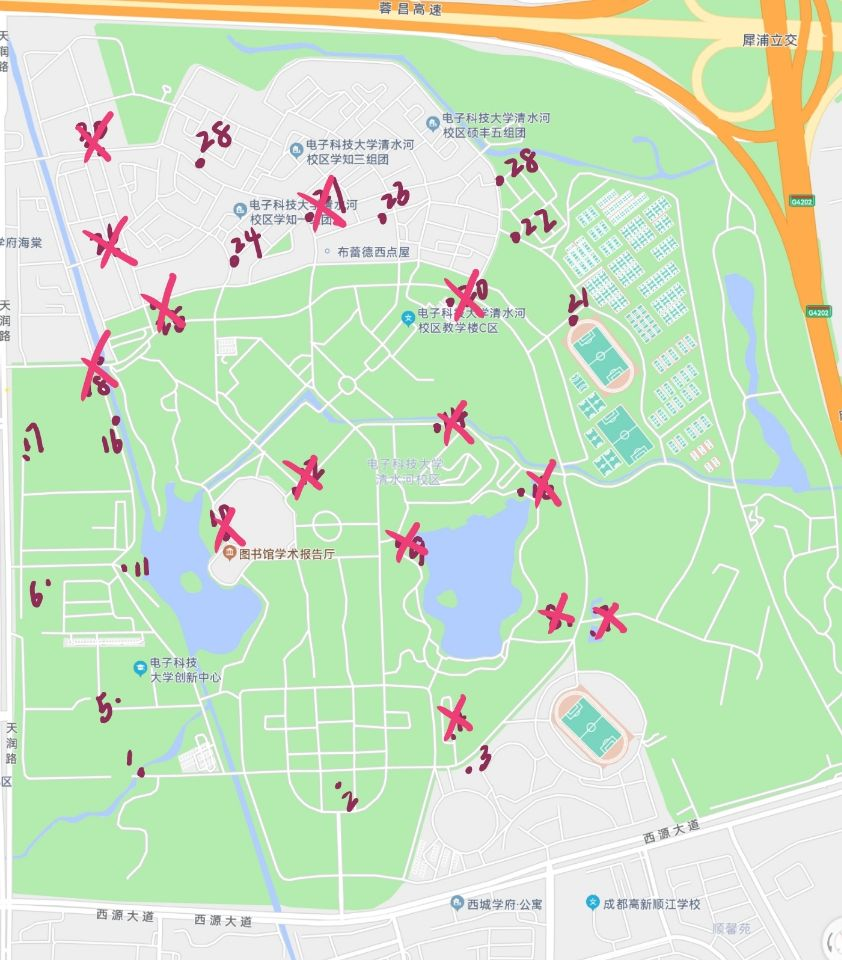
\includegraphics[width=0.4\textwidth]{pic7.jpg}
    %\caption{自卸车卸货的两个过程}
    \caption{取消与保留充电桩建设点位}
\end{figure}
\begin{figure}[H]
    \centering
    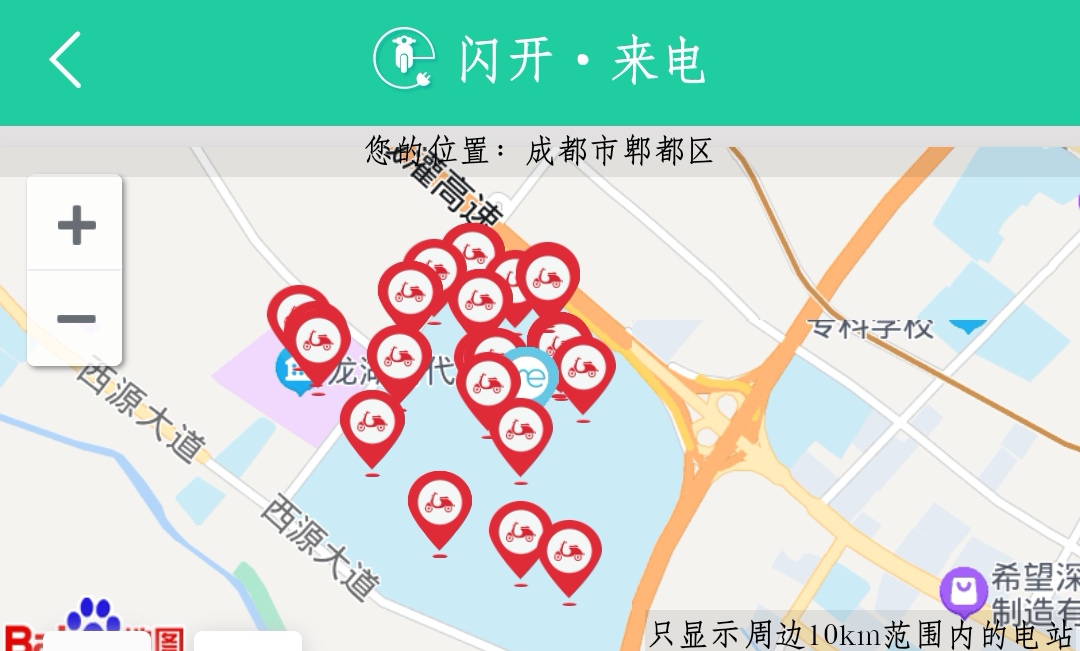
\includegraphics[width=0.6\textwidth]{pic1.jpg}
    %\caption{自卸车卸货的两个过程}
    \caption{与现有校园充电桩分布进行对比}
\end{figure}
与现有校园充电桩分布进行对比分析有:现有充电桩再商业街学生活动中心处布点过分密集,但在西门-西二门附近学生需求量较大区域布点明显不足。同时,在南门体育场附近布点冗余可以取消,其他位置布点合理与计算结果基本重合。